\chapter{Quantum Computing}

\section{Introduzione}

La rivoluzione scientifica che diede origine al corpo di conoscenze
che va sotto il nome di Fisica Quantistica ebbe luogo all’incirca nei
primi trenta/quaranta anni del XX secolo. Tra i protagonisti di questa rivoluzione, ricordiamo Max Planck,
Niels Bohr, Albert Einstein, Erwin Schr\"odinger, Louis de Broglie,
Werner Heisenberg, Paul Dirac, John von Neumann. Gli esperimenti condotti in quegli anni mostravano che, a livello
subatomico, la materia si comportava in modo radicalmente diverso
da come invece faceva a livello macroscopico, e gli scienziati
svilupparono opportuni formalismi matematici in grado di rendere
conto delle osservazioni sperimentali e delle nuove scoperte. A livello subatomico la materia manifesta proprietà e comportamenti
in molti casi bizzarri e controintuitivi, se confrontati con le proprietà
e i comportamenti che osserviamo a livello macroscopico (livello del
quale si occupa la fisica classica). 

\dfn{Fisica Quantistica}{
  La Fisica Quantistica è quella branca della fisica
che si occupa dello studio dei fenomeni fisici che hanno luogo
a livello atomico e subatomico.
}

\clm{}{}{
  \begin{itemize}
    \item A livello microscopico le entità atomiche e
subatomiche hanno un comportamento probabilistico, ciò significa
che il loro comportamento (per esempio la loro posizione in un certo
istante, o in che direzione e con che velocità si stanno muovendo) può
essere predetto solo con una legge probabilistica.
\item La formula matematica che riassume il comportamento probabilistico
di una entità atomica prende il nome di funzione d’onda, secondo la
teoria sviluppata da Erwin Schr\"odinger nel 1926.

  \end{itemize}
}

\dfn{Quantum Computing}{
  Col termine \newfancyglitter{Quantum Computing} si indica la disciplina all’intersezione tra Fisica Quantistica
e Informatica che studia come implementare algoritmi sfruttando
alcune caratteristiche manifestate dalla materia a livello subatomico.
}

\nt{Alcune di queste caratteristiche rendono le potenzialità della QC
molto promettenti, anche se dietro gli aspetti teorici si nascondono
difficoltà realizzative non ancora risolte in modo soddisfacente.}

\paragraph{Breve Recap:}

\begin{itemize}
  \item Nell’anno zero dell’era quantica, il 1900, Max Planck riesce
finalmente a modellare matematicamente il modo in cui i metalli,
riscaldati a diverse temperature, emettono una quantità ben precisa
di energia elettromagnetica. La soluzione di Planck
consiste nell’ipotizzare che
la radiazione elettromagnetica
(di cui la luce fa parte) venga
emessa dai metalli non in
modo continuo ma in
pacchetti di dimensione
prestabilita.
\item Nel 1905 Albert Einstein, sfruttando l’idea di Planck, spiega l’effetto
fotoelettrico ipotizzando una natura corpuscolare per la luce: le
particelle di luce (che verranno poi chiamate fotoni, o quanti di
luce), bombardano i metalli e strappano elettroni dalla loro superficie:
un fotone per ciascun elettrone.
\item Nel 1911 Ernest Rutheford, dopo aver scoperto che gli atomi sono
quasi completamente vuoti, ipotizza che assomiglino a microscopici
sistemi solari. 
\item Nel 1913 Niels Bohr, ricorrendo ancora all’idea dei pacchetti di
energia, spiega perché gli elettroni non precipitano sul nucleo fatto di
protoni: gli elettroni si muovono su orbite quantizzate, e possono spostarsi da
un’orbita all’altra solo assorbendo o emettendo un pacchetto di
energia (l’idea di “orbita” è ormai
superata, ma l’idea di stati quantici
rimane valida).
\item Negli stessi anni, lo studio del decadimento radioattivo e del
comportamento degli elettroni negli atomi mostra che atomi in
condizioni apparentemente identiche si comportano in modo diverso. Il loro comportamento può essere predetto solo facendo ricorso a
leggi probabilistiche. 
\item Intorno al 1922-1923, tutti i fisici sono più o meno convinti della
natura corpuscolare della luce: quando un fascio di luce attraversa un
gas, fotoni ed elettroni si scontrano fra di loro con un comportamento
simile a quello delle palle da bigliardo. 
\item Viene utilizzato un esperimento (delle due fenditure) per dimostrare che la luce possa essere contemporaneamente sia un'onda che un insieme di particelle.
\item Nel 1924, nella sua tesi di dottorato Louis de Broglie argomenta che
se le onde elettromagnetiche hanno anche una natura corpuscolare,
allora la materia può avere una natura ondulatoria, e mostra come
calcolare le lunghezze d’onda della materia. E infatti negli anni a venire l’esperimento a due fenditure sarà ripetuto
con elettroni, protoni, interi atomi, e infine con molecole complesse. 
\item La dicotomia classica che aveva regnato per centinaia di anni:
la realtà fisica fatta di materia e campi di forza, o equivalentemente,
particelle e onde, sembrava dissolversi in una unica “sostanza
quantica” che manifestava le proprietà di entrambe.
\begin{figure}[h]
    \centering
    
\includegraphics[width=0.3\textwidth]{05-QuantumComputing/meme.jpg}
    \caption{"È solo A o B ahhh rhetoric".}
\end{figure}
\item Tra il 1925 e il 1926 Werner Heisenberg, Erwin Schrödinger e
Paul Dirac formulano in modo indipendente addirittura tre modelli
matematici equivalenti in grado di descrivere e prevedere
il comportamento di questa “sostanza quantica”.
\end{itemize}

\section{Il Problema della Misurazione}

 La funzione d’onda associata ad una entità atomica o subatomica,
nota anche come equazione di Schr\"odinger codifica / sintetizza /
permette di calcolare, con un’unica espressione matematica:
\begin{itemize}
  \item Tutti i valori che possono assumere gli attributi di quella entità. 
  \item La probabilità con cui ciascun valore tra quelli possibili potrà
manifestarsi durante una misurazione.
\end{itemize}

La formulazione appena data, apparentemente semplice, nasconde al
suo interno alcune peculiarità singolari, che i fisici non hanno ancora
saputo spiegare, pur riuscendo a modellarle correttamente con un
appropriato formalismo matematico. Non a caso, uno dei grandi fisici del novecento, Richard Feynman (tra
l’altro il primo a intuire le potenzialità della quantum computing), ha
affermato che “nessuno capisce la fisica quantistica”, e prima di lui, a
Niels Bohr, uno dei padri della fisica quantistica, veniva attribuita
l’opinione secondo cui “lo scopo della scienza non era più di spiegare
la natura, ma solo di descrivere ciò che si può dire sulla natura”. Uno degli aspetti controintuitivi (e importante per la QC) ha
a che fare con il concetto di misura in fisica quantistica, dove
è fondamentale evitare di cercare paralleli con la fisica classica. 

\ex{La Fisica Classica}{
  Se sappiamo che una sfera di ferro si può trovare in uno di n
punti diversi dello spazio, nel momento in cui misuriamo la posizione
della sfera veniamo a conoscenza del punto specifico, tra gli n
possibili, in cui la sfera si trova. Ma diamo per scontato che la sfera fosse in quel particolare punto
anche immediatamente prima che la misurazione avesse luogo. In altre parole, la misurazione compiuta non ha alcuna influenza sul
sistema misurato, e il sistema viene lasciato nello stesso stato in cui
si trovava prima di essere misurato: dopo la misurazione la sfera si
troverà nello stesso punto in cui si trovava prima della misurazione. 
}

\ex{Fisica Quantistica}{
  In fisica quantistica le cose funzionano diversamente. Supponiamo
che un elettrone possa trovarsi in una di n posizioni possibili con
probabilità $c_0, c_1, … c_{n-1}$. Indichiamo con $X = [c_0, c_1, c_2, …c_{n-1}]$ lo
stato dell’elettrone. (dove sarà: $c_0 + c_1 + …+ c_{n-1} = 1$).

Questo non significa (come saremmo tentati di assumere), che
l’elettrone si trova in posizione $k$ con probabilità $c_k$.
Dire che il sistema è nello stato $X$ significa dire che l’elettrone si
trova contemporaneamente in tutte le possibili posizioni ammesse.

Fino a che non decidiamo di misurare la posizione dell’elettrone per
sapere dove si trova, dobbiamo accettare che l’elettrone si trovi
non in una delle posizioni possibili, ma in tutte: più propriamente
diciamo che l’elettrone si trova in una sovrapposizione di stati.

Sarà solo quando decideremo di effettuare una misurazione, che
troveremo l’elettrone in una specifica posizione. È solo nell’atto della
misurazione di un oggetto quantistico che la sovrapposizione di
stati in cui si trova collassa in un singolo stato in senso ordinario.

Ma prima di essere misurato, un sistema quantistico si trova
contemporaneamente in più stati, e in questo risiede il potenziale
della computazione quantistica: corrisponde ad avere un
computer capace di eseguire un algoritmo processando in
parallelo (un parallelismo reale, non simulato) tutti i possibili
input ammessi per quell’algoritmo.
}

\nt{In fisica quantistica dire che un sistema si trova nello stato $X$ significa dire che, solo
dopo averlo misurato, lo troveremo in posizione k con probabilità $c_k$.}

\subsection{Bit e Qubit}

Un bit ordinario descrive un sistema che può trovarsi in uno di due
possibili stati: aperto/chiuso, acceso/spento, vero/falso. I due stati in
cui si può trovare il sistema vengono di solito indicati con 0 e 1. Il formalismo matematico alla base della fisica quantistica fa un uso
esteso di matrici e vettori, dunque proviamo a usare quel formalismo
per rappresentare un bit ordinario a 0 oppure a 1 mediante matrici
2 x 1. Indicheremo il valore 0 con $|0>$ e il valore 1 con $|1>$. 

\nt{La notazione $|x>$, detta \fancyglitter{ket}, è stata introdotta da Paul Dirac. 
Possiamo leggere la notazione matriciale che abbiamo introdotto in
questo modo: $|0>$ significa che il bit si trova nello stato “0” con
probabilità 1, e si trova nello stato “1” con probabilità 0. $|1>$ significa
che il bit si trova nello stato “0” con probabilità 0 e nello stato “1” con
probabilità 1.
}

\clm{}{}{
  \begin{itemize}
    \item Usare probabilità per rappresentare bit “normali” è inutilmente
pesante, ma è perfetto per rappresentare un qubit, ossia un sistema
quantistico che può trovarsi in una di due possibili configurazioni:
0 e 1, con probabilità diverse. 
\item Poiché il sistema quantistico che rappresenta un qubit può assumere,
una volta misurato, uno di due valori possibili, descriviamo il
sistema mediante una matrice a valori complessi con due righe e una
colonna. 
\item Un qubit, fino a che non viene misurato, si trova
sempre in una sovrapposizione di due stati, corrispondenti ai valori 0 e
1. Alla misurazione, lo stato del qubit collasserà in uno dei due stati
possibili, trasformandosi così in un bit ordinario di valore 0 o 1.
\item non è possibile “vedere” un qubit, perché nel
momento in cui lo si osserva, ossia lo si misura, questo si trasforma in
un normale bit, con un valore ben preciso 0 o 1. Non di meno i qubit
esistono in un senso molto reale.
\end{itemize}
}

\subsubsection{}

Nei computer ordinari, un bit viene implementato mediante due livelli
di tensione diversi, associati alle due informazioni 0 e 1. Per costruire un qubit, nella quantum computing si sfruttano alcune
caratteristiche delle particelle subatomiche. Per esempio, un fotone
può trovarsi in uno di due possibili stati di polarizzazione, oppure un
elettrone è dotato di una caratteristica fisica chiamata spin che può
assumere due possibili valori diversi, che possiamo associare a 0 e 1.
Ogni stato di un sistema formato da 8 bit, ossia un qubyte deve
essere scritto con una matrice di
256 numeri complessi che soddisfano la proprietà:
$|c_0|^2 + … +|c_{106}|^2 + |c_{107}|^2 + |c_{108}|^2 + … + |c_{255}|^2
=1$

Dunque, nel mondo ordinario per indicare lo stato di un byte
dobbiamo scrivere in tutto 8 bit. Ma nel mondo dei quanti, lo stato di
otto qubit (appunto, un qubyte) deve essere descritto usando 256
numeri complessi, perché ognuna delle 256 combinazioni possibili
di 8 bit deve essere associata alla probabilità che ha di
manifestarsi, quando viene misurata. Se volessimo simulare su un computer ordinario un
computer quantistico dotato di un solo registro a 64 qubit avremmo
bisogno di poter memorizzare 264 numeri complessi, ossia più di 18
miliardi di miliardi di numeri complessi.
Assumendo di usare 8 byte per scrivere un numero reale, e dato che
ogni numero complesso è formato da una coppia di numeri reali,
questo corrisponde ad uno spazio di più di 288 milioni di terabyte.

\subsection{Porte Logiche}

Un computer è in definitiva un circuito logico estremamente
complesso, in cui dell’informazione in input scritta su $n$ bit viene
trasformata in informazione in output scritta su $m$ bit passando
attraverso un certo numero di porte logiche.
Gli $n$ bit di informazione in input possono essere rappresentati come una matrice di $2^n$ righe x 1 colonna, e gli $m$ bit di output saranno rappresentati con una matrice di
$2^m$ righe x 1 colonna (matrici con più righe e una colonna sono di
solito chiamate vettori colonna, cioè vettori rappresentati in verticale). Dunque rappresenteremo sequenze di bit mediante vettori colonna, e porte logiche mediante matrici.

È noto che qualsiasi circuito logico può essere formulato con una
opportuna combinazione di porte NOT e porte AND. La matrice NOT deve trasformare il vettore colonna $|0>$ nel vettore colonna $|1>$, e viceversa. Abbastanza intuitivamente poi, moltiplicando la matrice NOT per la matrice AND otteniamo la matrice corrispondente alla porta logica
NAND (ossia una porta AND con l’output negato da una porta logica NOT). La NAND è una porta logica universale: qualsiasi circuito logico
può essere costruito con una opportuna combinazione di porte logiche
NAND.

In maniera del tutto analoga, anche nella Quantum Computing la
computazione avviene usando porte logiche quantistiche, che
manipolano qubit in input per trasformarli in qubit di output. Le porte logiche quantistiche devono soddisfare alcune condizioni matematiche, ma a
parte questo, anche nella QC esistono particolari insiemi di porte
logiche quantistiche che sono universali, ossia possono essere
composte fra loro in opportune combinazioni e usate per eseguire
qualsiasi tipo di computazione.
Ma, pensando sempre alla descrizione di porta logica data mediante
una opportuna matrice, la differenza fondamentale tra una porta logica
ordinaria e una porta logica quantistica è che in quest’ultima la
matrice che la descrive può essere composta da numeri diversi da 0 e
1 (e nel caso più generale complessi).

\dfn{Matrice di Hadamard}{
  La \newfancyglitter{matrice di Hadamard}, che ha la proprietà di mettere
un qubit in input in una sovrapposizione di stati per cui il qubit di
output è per metà nello stato $|0>$ e per metà nello stato $|1>$.
}

\nt{In altre parole, se misuriamo ripetutamente il qubit $|0>$ lo troveremo
sempre nello stato 0. Se invece misuriamo ripetutamente il qubit $H|0>$ (a cui è stata applicata la matrice di Hadamard) lo troveremo metà delle volte nello stato 0 e lo troveremo metà delle
volte nello stato 1.}

\subsubsection{}
Proprio come nel caso classico, più porte logiche quantistiche
possono essere combinate assieme per portare avanti computazioni
più complesse. Ciò equivale a moltiplicare fra loro le matrici
corrispondenti. Ma notiamo una differenza fondamentale col caso classico: nel
momento in cui li misuriamo, i qubit si trasformano in bit ordinari,
e qualsiasi vantaggio della computazione quantistica scompare.
Se dovessimo effettuare la misurazione tra le porte A e B, la nostra
computazione quantistica si fermerebbe in quel momento.
Dunque, la misurazione va posticipata fino a quando non sono stati
eseguiti tutti i calcoli desiderati in modalità quantistica.

\dfn{Decoerenza Quantistica}{
  Le particelle subatomiche che implementano i qubit tendono spontaneamente a
interagire con l’ambiente circostante e, così facendo, in tempi
brevissimi si trasformano in bit ordinari e perdono l’informazione che
veicolavano.
}

\nt{Più è complesso il calcolo quantistico da portare avanti, maggiore è
il numero di porte logiche quantistiche da attraversare, e maggiore
sarà la probabilità che la decoerenza avvenga prima del
completamento del calcolo, vanificandolo. Mitigare questo problema
richiede soluzioni tecniche complesse e di difficile implementazione.}

\section{Algoritmi Quantistici}

Gli algoritmi quantistici non sono veri e propri algoritmi, almeno non
nel senso in cui normalmente intendiamo un algoritmo. Non esistono criteri generali per la scrittura degli algoritmi quantistici,
e la soluzione a un certo problema è sempre un po’ ad hoc, studiata
specificamente per quel problema e non immediatamente estendibile
ad altri problemi. 
Nei casi in cui l’algoritmo quantistico si dimostra inerentemente
superiore a una soluzione classica, ciò si deve alla possibilità di
sfruttare il concetto di sovrapposizione degli stati. In questo modo,
i diversi casi che un algoritmo classico dovrebbe considerare uno
per uno, nella versione quantistica possono essere processati tutti
insieme contemporaneamente.

\dfn{Algoritmo Quantistico di Deutsch}{
 L’algoritmo quantistico di Deutsch-Jozsa verifica una specifica
proprietà di alcune funzioni $\{0,1\}^n \Rightarrow \{0,1\}$. 

}


\nt{  L’algoritmo è costruito apposta per mostrare le potenzialità della
quantum computing. Nel caso generale però, la soluzione quantistica
di un problema non sempre è più efficiente di quella classica (e a volte
neppure si sa se esiste…). Inoltre, un algoritmo quantistico è molto
diverso da uno classico.
}

\pagebreak 
\subsubsection{}
Le funzioni sono in tutto quattro:

\begin{figure}[h]
  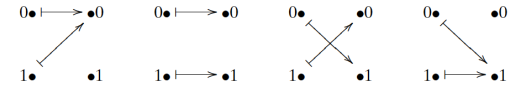
\includegraphics[scale = 0.5]{05-QuantumComputing/Deutsch.png}
\end{figure}
e data una funzione $f$: $\{0,1\} \Rightarrow \{0,1\}$ diciamo che $f$ è bilanciata
se $f(0) <> f(1)$, mentre diciamo che $f(x)$ è costante se $f(0) = f(1)$. Delle quattro funzioni possibili due sono bilanciate
e due sono costanti. L’algoritmo di Deutsch risolve il seguente problema: data una
funzione come black box (non possiamo cioè sapere
come è fatta dentro), determinare se è bilanciata o costante.
Il problema equivale a: data la black box con dentro $f$
determinare se corrisponde a una funzione bilanciata o costante.
Un algoritmo classico risolverebbe il problema più o meno così: 

\begin{itemize}
  \item Calcola $f(0)$.
  \item Calcola $f(1)$. 
  \item Confronta i due risultati.
\end{itemize}

\subsection{Il Funzionamento di un Algoritmo Quantistico}

\nt{Questa sezione è inserita solo per una questione di completezza, ma è molto tecnica e complicata.}
\subsubsection{}
Le porte logiche quantistiche devono essere
reversibili: dato un qualsiasi output deve sempre essere possibile
risalire all’input che lo ha prodotto. Nel caso della matrice: 

\begin{figure}[h]
    \centering
    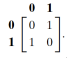
\includegraphics{05-QuantumComputing/a1.png}
\end{figure}
\subsubsection{}
e quindi della funzione: 

\begin{figure}[h]
    \centering
    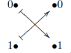
\includegraphics{05-QuantumComputing/a2.png}
\end{figure}
\subsubsection{}
il calcolo è reversibile, ma non lo sarebbe per: 

\begin{figure}[!h]
    \centering
    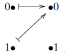
\includegraphics{05-QuantumComputing/a3.png}
    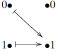
\includegraphics{05-QuantumComputing/a4.png}
\end{figure}

\subsubsection{}
Per implementare l’algoritmo di Deutsch abbiamo allora bisogno di
usare matrici un po’ più complesse, ma che corrisponderanno sempre
ai quattro casi della funzione f. Vediamo come costruire una porta
logica reversibile che calcoli il caso f(0) = 1; f(1) = 0. In modo
analogo si procederà per gli altri tre casi.
Consideriamo questo circuito quantistico:

\begin{figure}[h]
    \centering
    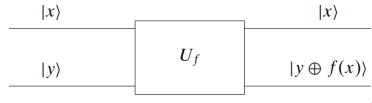
\includegraphics[scale=0.6]{05-QuantumComputing/a5.png}
\end{figure}

\subsubsection{}

Valutiamo l’output di questo circuito per i due possibili valori di y: 

\begin{itemize}
  \item Se y = 0, allora l’input $|x, 0>$ deve produrre:
    \begin{itemize}
      \item L’output $|0, 1>$ se x = 0. 
      \item L’output $|1, 0>$ se x = 1.
    \end{itemize}
  \item Se y = 1, allora l’input $|x, 1>$ deve produrre:
    \begin{itemize}
      \item L’output $|0, 0>$ se x = 0.
      \item L’output |1, 1> se x = 1.
    \end{itemize}
\end{itemize}
\subsubsection{}
Il che porta a definire la matrice $U_f$,
con i 4 input possibili sulle colonne e i 4 output
sulle righe: un 1 all’incrocio indica che quell’input
produce l’output corrispondente.
Che $U_f$ sia reversibile si può dedurre da questo circuito logico:
\begin{figure}[h]
    \centering
    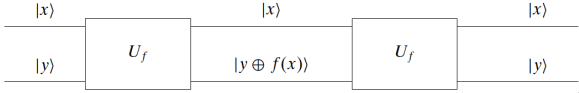
\includegraphics[scale=0.7]{05-QuantumComputing/a6.png}
\end{figure}
\subsubsection{}
L’output del circuito è:
$$|x, (y XOR f(x)) XOR f(x)> =
|x, y XOR (f(x) XOR f(x))> = |x, y XOR 0> = |x, y>$$
\subsubsection{}
Ossia, due applicazioni successive della porta logica $U_f$ restituiscono
l’input iniziale. E notiamo che $f(x)$ può essere sempre ricavata
dall’output di $U_f$, dato che: $y XOR f(x) XOR y = f(x) XOR 0 = f(x)$.
In modo analogo si possono costruire le $U_f$ delle altre 3 funzioni $f$.
Ecco qui di seguito un riassunto delle quattro funzioni $f$ possibili:
\begin{figure}[h]
    \centering
    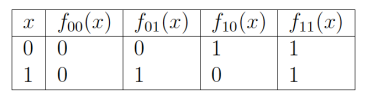
\includegraphics[scale=0.5]{05-QuantumComputing/a7.png}
\end{figure}
\subsubsection{}
e le quattro porte logiche quantistiche reversibili corrispondenti:
\begin{figure}[h]
    \centering
    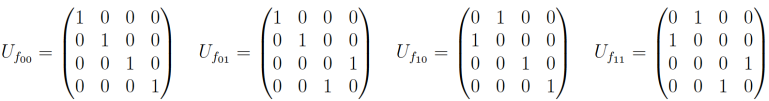
\includegraphics[scale=0.5]{05-QuantumComputing/a8.png}
\end{figure}
\subsubsection{}
Dunque, supponiamo che sia $U_f$ la matrice che ci viene data, che è
una della quattro $U_f$ possibili (e nel caso generale noi non sappiamo
quale), e consideriamo questo circuito quantistico:
\begin{figure}[h]
    \centering
    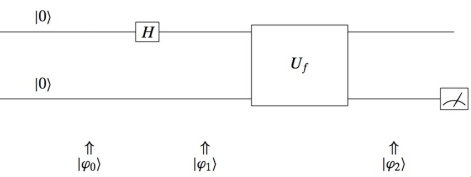
\includegraphics[scale=0.5]{05-QuantumComputing/a9.png}
\end{figure}
\subsubsection{}
Dove H è il segnale di misurazione, e il simbolo in basso a destra è la misurazione finale.
Inizialmente il sistema è nello stato:
\begin{figure}[h]
    \centering
    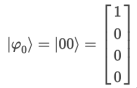
\includegraphics[scale=0.5]{05-QuantumComputing/a10.png}
\end{figure}
\subsubsection{}
Il qubit superiore, ossia l’input $|x>$ viene messo dalla matrice di
Hadamard in una sovrapposizione di stati, e dunque avremo:
\begin{figure}[!h]
    \centering
    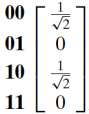
\includegraphics[scale=0.5]{05-QuantumComputing/a11.png}
\end{figure}
\subsubsection{}
E dopo aver applicato la matrice $U_f$, nel caso specifico di $f = f_{10}$,
avremo:

\begin{figure}[!h]
    \centering
    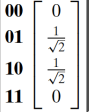
\includegraphics[scale=0.5]{05-QuantumComputing/a12.png}
\end{figure}

\nt{Ma se anche ora misuriamo più volte il qubit superiore in output lo
troveremo il 50\% delle volte nello stato $|0>$ e il 50\% delle volte nello
stato $|1>$, e la stessa cosa per il qubit inferiore, dunque, così com’è,
questo circuito non sembra molto utile a risolvere il problema.}
\subsubsection{}
Proviamo allora con un algoritmo leggermente diverso:

\begin{figure}[!h]
    \centering
    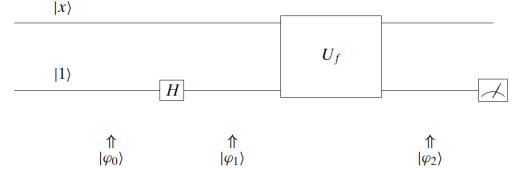
\includegraphics[scale=0.5]{05-QuantumComputing/a13.png}
\end{figure}
\subsubsection{}
Dopo l’applicazione di $U_f$, avremo:
\begin{figure}[!h]
    \centering
    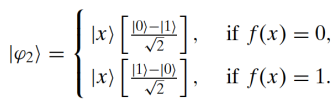
\includegraphics[scale=0.5]{05-QuantumComputing/a14.png}
\end{figure}

\nt{Ma di nuovo, se valutiamo i qubit non otteniamo
molto: il qubit superiore sarà nello stato $|x>$ e troveremo il qubit
inferiore nello stato $|0>$ o nello stato $|1>$}
\subsubsection{}
Ma è combinando i due tentativi precedenti che otteniamo l’algoritmo
di Deutsch: la soluzione consiste nel mettere entrambi i qubit di input
in una sovrapposizione di stati attraverso la matrice di Hadamard,
e così pure per l’output superiore:
\begin{figure}[!h]
    \centering
    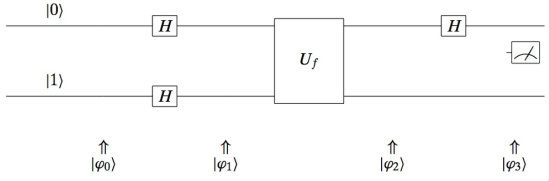
\includegraphics[scale=0.5]{05-QuantumComputing/a15.png}
\end{figure}

\subsubsection{}
Da 
\begin{figure}[!h]
    \centering
    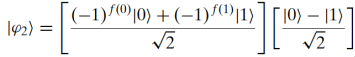
\includegraphics[scale=0.5]{05-QuantumComputing/a16.png}
\end{figure}
\subsubsection{}
Consideriamo ora la parte di espressione:
\begin{figure}[!h]
    \centering
    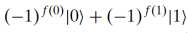
\includegraphics[scale=0.5]{05-QuantumComputing/a17.png}
\end{figure}

\begin{itemize}
  \item Se $f$ è costante, ossia se $f(0) = f(1)$, allora l’espressione si riduce a:
    \begin{itemize}
      \item $+1(|0> + |1>)$ se $f(0) = f(1) = 0$.
      \item $–1(|0> + |1>)$ se $f(0) = f(1) =1$.
    \end{itemize}
  \item Se $f$ è bilanciata, ossia se $f(0 <> f(1))$, allora l’espressione si riduce a:
    \begin{itemize}
      \item $+1(|0> – |1>)se f(0) = 0$ mentre $f(1) = 1$.
      \item $–1(|0> – |1>)se f(0) = 1$ mentre $f(1) = 0$.
    \end{itemize}
\end{itemize}

\subsubsection{}
Mettendo insieme i quattro casi abbiamo:

\begin{figure}[!h]
    \centering
    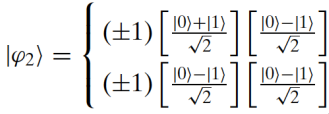
\includegraphics[scale=0.5]{05-QuantumComputing/a18.png}
\end{figure}
\subsubsection{}
Dopo l’applicazione della matrice di Hadamard al qubit
superiore, avremo:
\begin{figure}[!h]
    \centering
    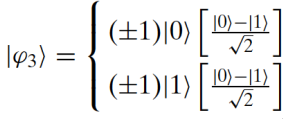
\includegraphics[scale=0.5]{05-QuantumComputing/a19.png}
\end{figure}
\subsubsection{}
A questo punto ci basta misurare il qubit superiore: se lo troviamo
nello stato $|0>$ sappiamo che abbiamo a che fare con una funzione $f$
costante, se lo troviamo nello stato $|1>$ sappiamo che $f$ è bilanciata.

\nt{Non è assolutamente evidente a priori perché il circuito
quantistico usato dovrebbe funzionare, e questo è tipico del modo di
progettare algoritmi quantistici, e criteri generali come quelli usati
per gli algoritmi classici non esistono}

\subsection{Altri Algoritmi Quantistici}

\begin{itemize}
\item \fancyglitter{Algoritmo di Simon}: è in grado di trovare pattern che si ripetono in
funzioni del tipo $f: {0,1}n \Rightarrow {0,1}n$. Mentre un algoritmo classico
risolve il problema in tempo proporzionale a $2^n$ chiamate di $f$,
l’algoritmo di Simon lo risolve in tempo proporzionale a n chiamate.
\item \fancyglitter{Algoritmo di Grover}: sia data una funzione $f$ che riceve in input $n$ bit
e restituisce 1 per una sola delle $2^n$ possibili combinazioni in input.
L’algoritmo di Grover è in grado di trovare la combinazione $x$ per cui
$f(x) = 1$ con un numero di interrogazioni di $f$ pari a $\sqrt[2][2^n]$.
\item \fancyglitter{Algoritmo di Shor}: la sicurezza della crittografia a chiave pubblica è
data dalla difficoltà di dedurre la chiave privata da quella pubblica. In
altre parole, la difficoltà di fattorizzare un numero molto grande (ossia
trovare l’insieme di numeri primi il cui prodotto dà il numero stesso).
L’algoritmo di Shor è in grado di fattorizzare un numero N in un
tempo proporzionale a $(log N)^3$.
\end{itemize}

\section{Computer Quantistici}

La costruzione di computer quantistici attraverso cui implementare le
idee teoriche che abbiamo visto va avanti ormai da più di 25 anni. Diverse tecniche sono state sperimentate e diverse soluzioni adottate
per superare le difficoltà che si presentano quando si ha a che fare con
il comportamento bizzarro della materia nell’infinitamente piccolo. 
Innanzi tutto, occorre implementare il concetto di qubit, e come già
accennato, diverse opzioni sono possibili, ciascuna con i propri pregi
e i propri difetti. Possiamo usare lo spin degli elettroni, la polarizzazione dei fotoni, lo
stato di eccitazione degli atomi, e molto altro ancora. Ogni opzione
richiede di risolvere problemi tecnici molto complessi (per esempio,
mantenere i circuiti a temperature vicine allo zero assoluto)

Un problema molto serio che qualsiasi implementazione deve
risolvere è quello della decoerenza, per cui il mezzo fisico usato per
implementare i qubit perde l’informazione memorizzata a causa
dell’interazione con l’ambiente circostante.
Per far partire una computazione quantistica abbiamo bisogno di un
certo numero di qubit inizializzati in una configurazione di input:
ad esempio elettroni tutti con lo spin nello stesso verso, corrispondenti
ognuno al qubit $|0>$. Il problema è che questi elettroni incominceranno immediatamente
ad interagire con l’ambiente circostante, e con i miliardi di miliardi
di elettroni di cui è composto, secondo un fenomeno noto ai fisici col
termine di \fancyglitter{entaglement}. A causa dell’entanglement ha luogo la decoerenza: l’informazione
trasportata dai qubits viene modificata in modo imprevedibile, con
conseguenti errori nella computazione. Purtroppo, non è così ovvio
sapere se, durante un calcolo, si sia verificata o meno la decoerenza. Vi sono sostanzialmente tre modi per cercare di minimizzare il
problema della decoerenza:

\begin{itemize}
  \item A seconda delle implementazioni, la decoerenza si verifica più o
meno tra i 100 microsecondi e alcuni secondi dalla fase di
inizializzazione dei qubit nella configurazione di partenza, e dunque
l’idea è di cercare di portare a termine la computazione quantistica
prima che si verifichino la decoerenza e gli errori di calcolo.
\item Usare una qualche forma di correzione degli errori, ossia usare alcuni
qubit per correggere eventuali errori introdotti dalla decoerenza di
altri qubit. 
\item Ripetere più volte un calcolo e scegliere poi “a maggioranza” il
risultato giusto.
\end{itemize}

\nt{Questi metodi non si escludono a vicenda: il progresso
tecnologico cerca allo stesso tempo di tenere la decoerenza sotto
controllo, e di costruire computer quantistici dotati di un maggior
numero di qubits, una parte dei quali verrà usata per la correzione
degli errori.}
\clm{}{}{
  \begin{itemize}
    \item I computer quantistici attuali sono in grado di operare su un numero
di qubit che arriva attualmente ai 105 qbit di Google (il precedente
Sycamore ne usava 72), ma questi numeri hanno poca o nessuna
relazione con i corrispondenti numeri di un computer classico, e i
confronti sono improponibili. 
\item Dei qubit disponibili, alcuni devono essere usati per correggere
eventuali errori, e si può dimostrare che un singolo qubit logico
deve essere implementato con non meno di 5 qubit effettivi per
poter correggere qualsiasi errore dovuto alla decoerenza.
  \end{itemize}
}

\subsection{Quantum Supremacy}

Nell’autunno del 2019 Google annunciava di aver raggiunto la
Quantum Supremacy: il Sycamore, aveva effettuato in circa 200
secondi un calcolo che avrebbe richiesto più di diecimila anni al
super computer Summit della IBM. A giugno 2020 il Summit risultava essere il secondo supercomputer
più potente al mondo, con una potenza di calcolo di circa 200.000
Teraflop al secondo. I ricercatori della IBM replicarono all’annuncio
di Google che Summit, dotato di una quantità maggiore di memoria di
massa (attualmente ha quasi 3 milioni di Gigabyte) avrebbe risolto lo
stesso problema in 2 giorni e mezzo, e con maggiore precisione, e che
dunque la presunta supremazia quantistica non era affatto stata
raggiunta.

\begin{figure}[!h]
    \centering
    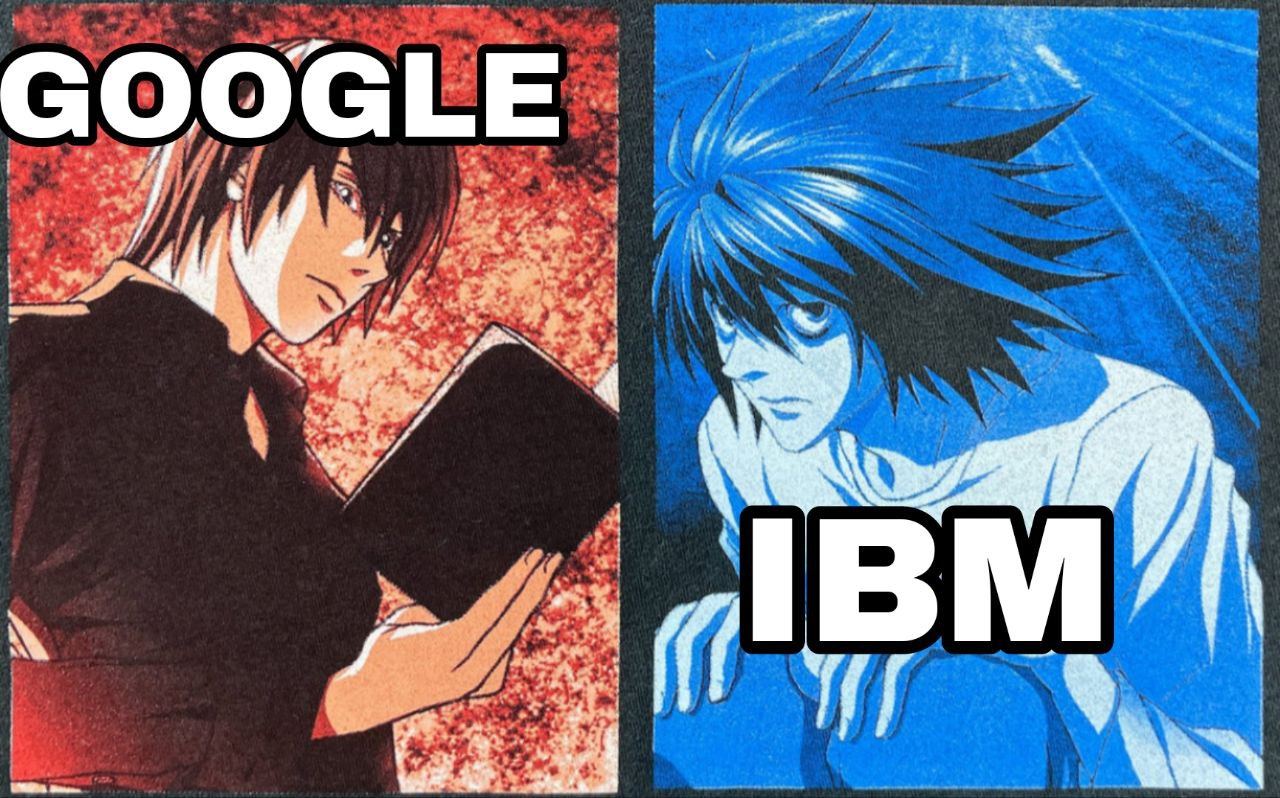
\includegraphics[scale=0.25]{05-QuantumComputing/meme2.jpg}
    \caption{"Questa non è la \textbf{\textit{supremazia quantistica}}, è soltanto l'opera di una \textbf{\textit{corporation infantile}} che crede di poter giudicare gli altri come se fosse Dio" - un ricercatore di IBM, probably.}
\end{figure}
\subsubsection{}
Il punto controverso sta nella famigerata Quantum Supremacy,
definita (nel 2012, da John Preskill) come l’obiettivo di dimostrare
che un computer quantistico può risolvere un problema che nessun
computer classico potrebbe risolvere in tempi ragionevoli.
Tuttavia, la definizione di supremazia quantistica è insoddisfacente, in
quanto non dice nulla sull’utilità del problema risolto, che quindi può
anche essere costruito ad arte per essere particolarmente vantaggioso
per un computer quantistico e particolarmente svantaggioso per un
computer classico (l’algoritmo di Deutsch-Josza ne è un esempio). E la definizione è fuorviante in quanto tende erroneamente a suggerire
che indichi il momento in cui i computer quantistici avranno superato
in prestazioni i computer classici indipendentemente dal problema da
risolvere. Allo stato attuale della ricerca, per applicazioni pratiche, la
computazione quantistica risulta effettivamente superiore a quella
classica solo per quei problemi in cui si può sfruttare il fenomeno
della sovrapposizione degli stati (per esempio in crittografia e per la
simulazione di sistemi quantistici). E in ogni caso, rimangono ancora da risolvere molti dei problemi
pratici relativi alla difficoltà di costruire e far funzionare
adeguatamente un computer quantistico, e i problemi relativi alla
gestione degli errori introdotti durante una computazione quantistica. Sono ormai in molti a pensare che la computazione quantistica non
sostituirà mai completamente quella classica, sia per la difficoltà di
costruire e usare computer quantistici usabili dal grande pubblico e
sia perché per molti problemi, non sembrano esistere (o almeno non
sono ancora state trovate) soluzioni quantistiche superiori a quelle
classiche. Al contrario, in molti sono convinti che lo scenario più probabile sarà
quello in cui computer quantistici e computer classici lavoreranno
insieme in modo da sfruttare di ciascuno le caratteristiche in cui
eccellono e i rispettivi punti di forza. In effetti, per molti algoritmi è
già così, e vengono implementati integrando una parte quantistica con
una classica (è il caso dell’algoritmo di Shor). 

\nt{Sono disponibili pochi dettagli tecnici su come sono costruiti i computer quantistici perché: 
\begin{itemize}
  \item In parte perché è una ricerca di frontiera. 
  \item In parte perché le corporation ci tengono ai loro segretini. 
\end{itemize}}
